
\documentclass[11pt]{article} % use larger type; default would be 10pt

\usepackage[utf8]{inputenc} % set input encoding (not needed with XeLaTeX)

%%% PAGE DIMENSIONS
\usepackage{geometry} % to change the page dimensions
\geometry{a4paper} % or letterpaper (US) or a5paper or....
% \geometry{margin=2in} % for example, change the margins to 2 inches all round
% \geometry{landscape} % set up the page for landscape
%   read geometry.pdf for detailed page layout information

\usepackage{graphicx} % support the \includegraphics command and options

% \usepackage[parfill]{parskip} % Activate to begin paragraphs with an empty line rather than an indent

%%% PACKAGES
\usepackage{booktabs} % for much better looking tables
\usepackage{array} % for better arrays (eg matrices) in maths
\usepackage{paralist} % very flexible & customisable lists (eg. enumerate/itemize, etc.)
\usepackage{verbatim} % adds environment for commenting out blocks of text & for better verbatim
\usepackage{subfig} % make it possible to include more than one captioned figure/table in a single float
% These packages are all incorporated in the memoir class to one degree or another...

%%% HEADERS & FOOTERS
\usepackage{fancyhdr} % This should be set AFTER setting up the page geometry
\pagestyle{fancy} % options: empty , plain , fancy
\renewcommand{\headrulewidth}{0pt} % customise the layout...
\lhead{}\chead{CS 5150 Feasibility Report: Sun in the City Group}\rhead{}
\lfoot{}\cfoot{\thepage}\rfoot{}

%%% SECTION TITLE APPEARANCE
\usepackage{sectsty}
\allsectionsfont{\sffamily\mdseries\upshape} % (See the fntguide.pdf for font help)
% (This matches ConTeXt defaults)

%%% ToC (table of contents) APPEARANCE
\usepackage[nottoc,notlof,notlot]{tocbibind} % Put the bibliography in the ToC
\usepackage[titles,subfigure]{tocloft} % Alter the style of the Table of Contents
\renewcommand{\cftsecfont}{\rmfamily\mdseries\upshape}
\renewcommand{\cftsecpagefont}{\rmfamily\mdseries\upshape} % No bold!

%%% END Article customizations

%%% The "real" document content comes below...

\title{CS 5150 Feasibility Report: Sun in the City Group}
\author{Phillip Tischler (pmt43), Brian Toth (bdt25), Vera Khovanskaya (vdk9), \\ 
Sean Salmon (ss2669), Lin Xue (lx39), Zach Porges (zip2),  \\
and James McGuinness (jrm369)}
%\date{} % Activate to display a given date or no date (if empty),
         % otherwise the current date is printed 

\begin{document}
\maketitle


\section{The Team (Skills and Experience)}

The team has a diverse background of technical knowledge as well as leadership and project experience. It has been determined that the backgrounds are more than sufficient to tackle this project. All members have familiarized themselves with the core technologies of the project prior to the feasibility study in order to talk intelligently about the topic. That is, each member has become familiar with HTML, CSS, PHP, MySQL, setting up a web server (Apache web with PHP and MySQL), and setting up Drupal.

\textbf{Phillip Tischler (pmt43@cornell.edu)}. Phillip is currently the Team Lead of an engineering project team at Cornell (CUAir, Cornell University’s Unmanned Air Systems Team) which includes managing development of 36 engineers. Previous to this position he was the Software Sub-team Lead and managed 8 software developers. His relevant experience in industry is when he lead development of a team of two other full time employees to create web software to manage large scale database and data processing engines, of which the software was deployed internally to approximately 100 operations employees.

\textbf{Brian Toth (bdt25@cornell.edu)}. Brian has programmed in Java, C, C\#, and Clojure. He has worked with Linux, Windows, and Git. His relevant experience includes developing an image-processing plugin for a large commercial software platform, and creating data acquisition software for an off-road racing vehicle for an engineering project team at Cornell (Cornell Baja SAE). His notable CS coursework includes 5414 (Distributed Computing), 5412 (Cloud Computing), 5430 (System Security), 5780 (Machine Learning), and 5620 (Intro Computer Graphics). He is currently a TA for CS 4410/4411 (Operating Systems).

\textbf{Vera Khovanskaya (vdk9@cornell.edu)}. Vera is an expert at visual prototyping software, Adobe Photoshop, Adobe Fireworks, and Adobe Illustrator. She has been researching Human-Computer Interaction for 2.5 years and has extensive experience with usability testing, role-play, and case analysis. In this research she has deployed and tested mobile health software, conducted open-ended interviews, and done design and prototyping work. In addition, she is fluent with HTML, CSS, and PHP.

\textbf{Zach Porges (zip2@cornell.edu)}. Zach is our team’s expert in HTML, CSS, PHP, MySQL, and mobile application design. He has developed web applications for the Ithaca Innovation Firm, a student run web and logo design firm. He is currently the TA for INFO 1300 (Intro to Design and Programming for the Web) and INFO 2300 (Intermediate Design and Programming for the Web).

\textbf{Sean Salmon (ss2669@cornell.edu)}. Sean has extensive experience with Java programming, HTML, constraint modeling, and statistical data analysis. He has completed CS 1110 and CS 2110. Currently Sean is working on CURB Website Design and has obtained experience with DreamWeaver and CSS.

\textbf{Lin Xue (lx39@cornell.edu)}. Lin is an experienced programmer with Java, Python, and C. He also has skills in Adobe Photoshop, Adobe Illustrator, Google SketchUp, and AutoCAD. In addition, he is also proficient in data analysis and is familiar with Mathematica and Origin. Lin has researched for over 4 years and has obtained experience with experimental physics in nanoscale magnetic devices, he has designed data acquisition software (LabWindows) as well as data analysis software (Python). He has published journal papers and given conference presentations.

\textbf{James McGuinness (jrm369@cornell.edu)}. James is proficient with Java, C, C++, OCaml, and Python. He’s worked with the Windows API and has experience via a variety of small projects done out of interest, as well as larger scale projects from CS 3110 and CS 3410. He also has some experience with statistical aggregation from previous projects.

\section{The Client}

The client for this project is The Cornell Daily Sun, a for-profit organization with its operations being run independently from Cornell since 1880. Currently the Cornell Daily Sun is the main source of news on campus regarding issues related directly to Cornell University students. The organization has both a print newspaper and an online newspaper, and generates revenue with the placement of advertisements. The points of contact in The Cornell Daily Sun are IT Manager Joseph Staehle, and Editor in Chief Juan Forrer.  Mr. Staehle presented the proposal and will be the primary client and point of contact for this project.

\begin{figure}[h]
\begin{center}
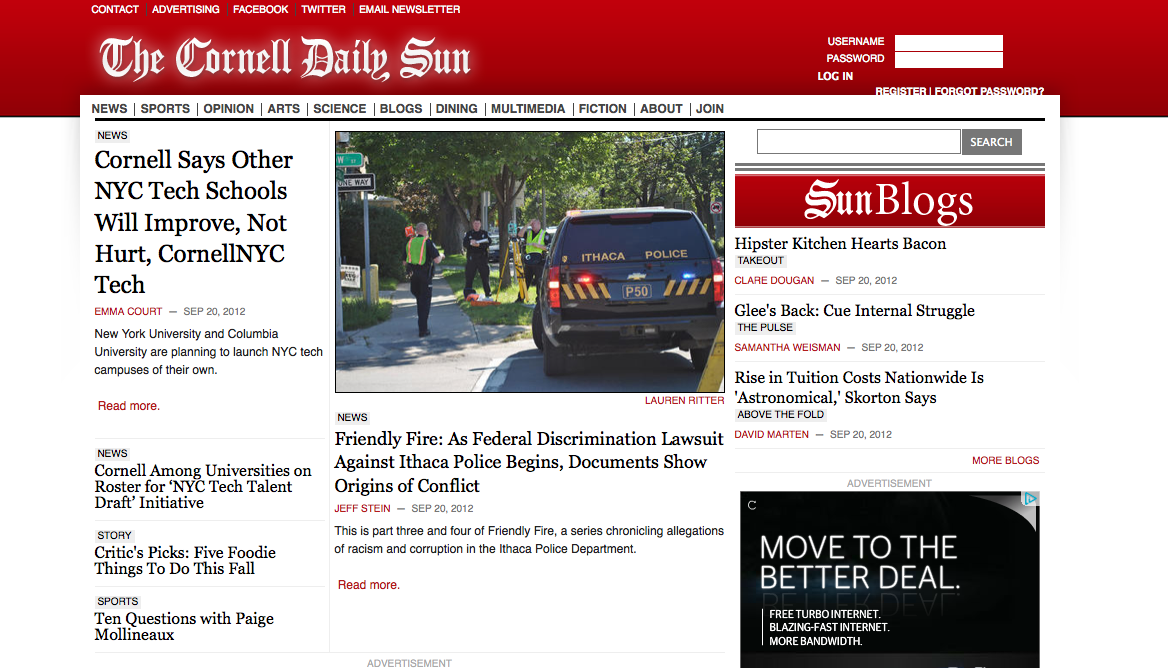
\includegraphics[width=6in]{images/cornell_sun_current}
\end{center}
\caption{The Cornell Daily Sun's Current Website}
\end{figure}

\subsection{Availability}

In regards to availability, Mr. Staehle is a student at Cornell University and resides on campus, and thus his schedule aligns with that of our teams which makes scheduling client-group meetings simple. Additionally, The Cornell Daily Sun is located in the Commons of Ithaca which is less than five minutes walk from Cornell campus. Prior to the completion of this feasibility report we will have met with the Editor in Chief once and our primary contact, Mr. Staehle, five times.

\subsection{Concerns}

The client has demonstrated to the team the commitment to seeing this project through its development and deployment. However, one concern was raised during the meetings. The success of the project post deployment relies on generating content writers as well as readers of the website, a task that can only be solved by the client. This raises two issues. First, The Cornell Daily Sun does not currently have writers for the proposed project. Secondly, generating a critical mass of website readers may be more difficult than expected. On a quarterly basis, The Cornell Daily Sun’s current website has approximately 80,000 unique visitors. This newspaper caters to the Cornell student population, a user base of approximately 13,000 undergraduates and 2,000 graduates. The difference in number of visitors is likely due to a vast pool of alumni that also read the website. The project proposed is one for the new Cornell Tech Campus, a campus that does not yet have an alumni populus to bridge the gap in number of readers. This concern has been voiced to the client, and steps to mitigate the issues are being taken. That is, The Cornell Daily Sun is now in the process of recruiting writers and determining how long it would take to obtain the critical mass of readers.

\section{Scope of Project}

The project analyzed in this document is one to build a new website and Content Management System (CMS) for The Cornell Daily Sun. This website will represent a new market for the client. That is, the client is attempting to expand its newspaper to begin bringing news to the students of Cornell University’s new Tech Campus in New York City.

\subsection{System Status}

The Cornell Daily Sun website is an existing product that is managed with a Drupal CMS and custom extensions. This project is to build a new website for the Cornell Tech Campus, and is therefore a new product and not an augmentation or replacement. However, if this new website is extremely successful the old website may be converted to the new one. To maintain familiarity with the CMS system, the client has requested the CMS be based off the Drupal CMS.

\subsection{Functionality}

There are four required pieces of functionality the project must support: a website for readers to browse the newspaper, a CMS to manage the website and allow writers to post content, a means to allow Data Fusion to present external content inline with content generated by The Cornell Daily Sun, and finally a Brand to associate with this new website. Like the existing CMS The Cornell Daily Sun uses, the CMS must allow the writers and editors to upload their content like articles, blogs, comments, images, and advertisements. The website itself must display this content in a reasonable and convenient way that allows readers to browse and obtain the information they are looking for. To create a unique Cornell Tech campus newspaper, the project also requires the team to create a Brand. This includes a logo, a display name, and a look and feel for this newspaper. A key aspect of this Brand will be Data Fusion, a distinction from the current website the client operates. Data Fusion will present articles from external sources inline with an article posted by the Cornell Daily Sun. It is similar to a “Read More” link, except this information will be external and automatically presented with the article from The Cornell Daily Sun.

There are three desired but not required pieces of functionality for the project: an optimized mobile version of the site, an algorithm to perform the Data Fusion automatically, and a performance optimizer for the entire system. The mobile optimized site will allow readers to browse The Cornell Daily Sun’s website on a mobile device in a much faster and convenient way than to load the main page onto a slower device with less screen display area. This functionality may require too much time to implement, which is why it is not a required portion of this project. The Data Fusion described in the paragraph above was a framework to allow custom algorithms to link external content as well as manually link content. The other piece of functionality that is not required is an algorithm to automatically detect and link external content to the content generated by The Cornell Daily Sun. This may involve web and RSS feed scraping as well as Machine Learning and other advanced topics. Due to the complexity of the functionality relative to the timeframe of the project, this functionality has been deemed not required. However, if implemented it will save time, make running the website easier, and increase the attractiveness to potential readers as it will dynamically update the site. The final desired but optional piece of functionality is a performance optimization that will decrease the time it takes to load the website. Using a 50Mbps connection (an average user only has access to a 2Mbps connection), the client’s current site takes over 5 seconds to load the visible page of the homepage and over 13 seconds to load the entire page. Most websites can respond in under 200 milliseconds and load completely in a second. Every millisecond the user waits has a psychological impact on their perception of the website, and thus it is critical to load as fast as possible. There are simple upgrades to the system that can be employed to achieve this goal. However, time and budget may be a limiting factor, which is why this functionality is desired but not required.

\begin{figure}[h]
\begin{center}
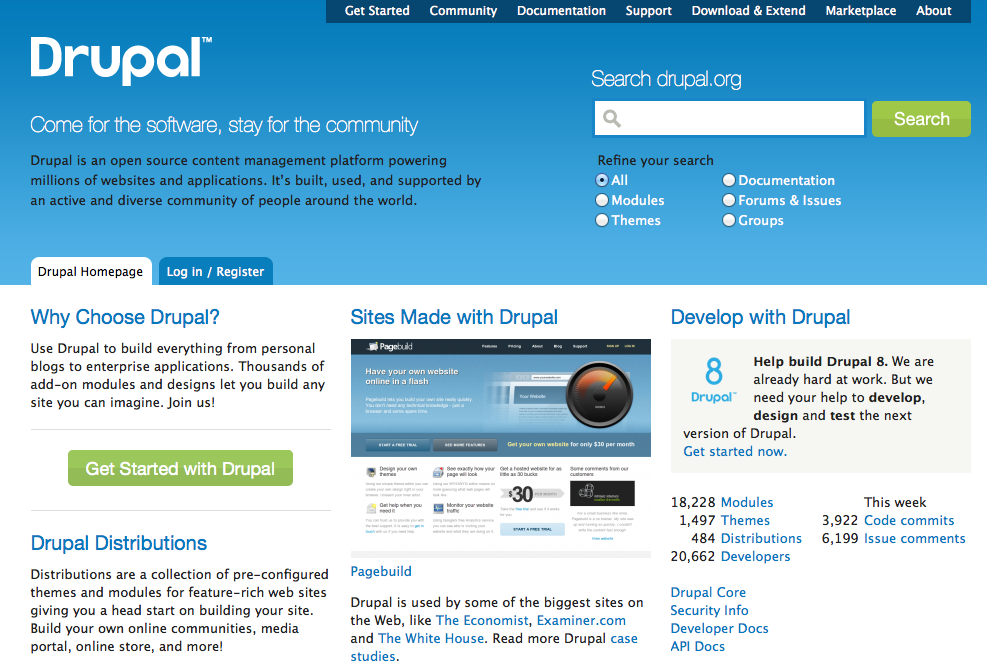
\includegraphics[width=6in]{images/drupal}
\end{center}
\caption{The Drupal CMS At Work}
\end{figure}

\subsection{Actors and their Use Cases}

\textbf{Reader}. Readers are the consumers of both the primary and secondary content on the website. They will generate the bulk of traffic to the system as there are orders of magnitude more readers as other types of actors. The use case they will primarily exercise is that of reading content on the website. They can find this content by either searching for it or browsing the various categories. It will be important to build trust with these users so that they desire to engage with the main content and with the secondary sources that we hope to integrate. Our own experiences with news content align most closely with this use-case, so we hope to accomplish preliminary usability testing on ourselves; however, as we grow more accustomed to the interface as developers, it will become increasingly important to test this use case on external audiences. This use case is of primary interest as it will define the success or failure of our client as these external stakeholders will generate the revenue.

\textbf{Editor}. This is that actor that represents our clients, and is of high priority because they will have the most responsibilities and most investment when interacting with the system. Editors exercise the use cases of editing content posted by writers, determining which content should be posted to the website, and approving the Data Fusion sources. Editors are the executors of the newspaper’s broader vision, and the intermediaries between the writers and the users. Editors will also need to understand how to maintain the system, and will be particularly sensitive to the various data fusion and machine learning algorithms the team may be implementing. It is important to consider the editors' needs in usability testing because they are the "keystone species" of this news content ecology.

\textbf{Writer}. The writers are the actors that generate primary content for the website and then decides what kind of secondary data, like Data Fusion sources, to include in their specific contribution. The use cases that writers go through are important to test because these actors are likely to be the less familiar with the system as they are least invested with The Cornell Daily Sun, and yet the most tech-savvy of our three actors as they will be generating content for a newspaper that is technical in nature.


\begin{figure}[h]
\begin{center}
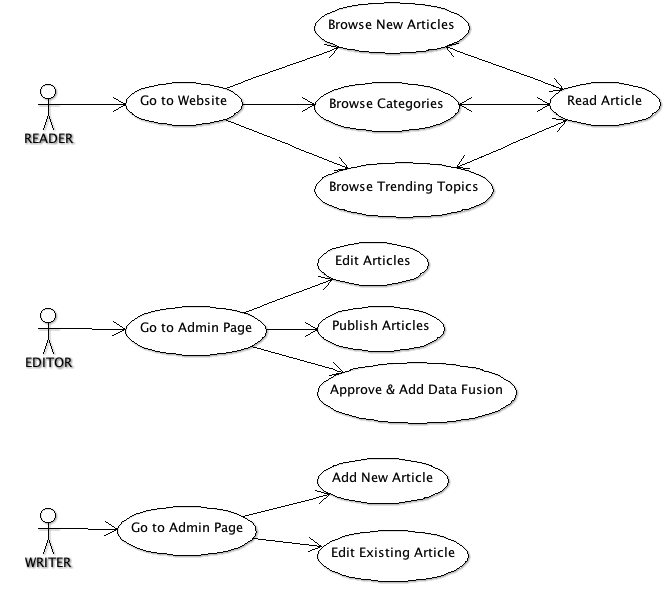
\includegraphics[width=4in]{images/use_case}
\end{center}
\caption{The Use Cases}
\end{figure}

\subsection{Dependencies}

\textbf{Drupal}. Drupal is an open-source CMS that The Cornell Daily Sun uses for their current website, and as such the CMS that will be used for this project. The Drupal CMS is licensed under the GNU General Public License. This license is explained under the discussion of business considerations. Drupal is composed PHP, HTML, and CSS to generate and display the content, and a MySQL database to store the information composing the content itself. Drupal 6 requires PHP 4.4.0 or higher, while Drupal 7, the latest release, will be used and it requires PHP 5.2.5.  Drupal provides a large baseline of features for a website, including but not limited to, user account handling, layout management, website menu customization, RSS feed aggregation, article search, and FTP access.  Extensions can be written for Drupal in PHP, and there are over 17,000 free extensions available that are also under the GNU General Public License. For this project, Drupal will provide a very strong base for building this system.

\textbf{Deployment Server}. We will be using a Linux-based server hosted on a cloud platform for purposes of development and eventually deployment. The plan is to use Amazon AWS as the cloud provider. Because Drupal uses PHP and MySQL only, a Linux server is appropriate.

\textbf{Data Fusion}. The Data Fusion extension will most likely be integrated into Drupal using a PHP module, but the core functionality of the scraper will be written in Java. Because Drupal already has RSS aggregation, it is very likely that the module will rely on some form of RSS news scraping to find similar news articles.

\section{Project Benefits}

There are two unique stakeholder entities that will benefit this project. The first is The Cornell Daily Sun that will own the product that results from the project. The second is the students and other community members of Cornell University's new Tech Campus. Each entity will benefit in different ways from the success of this project.

\subsection{Cornell Daily Sun}

With the new website, The Cornell Daily Sun will both expand its market, increase its influence, and increase its revenue. This project will allow the client to new types of content for both its paper based and web based publications. As the website matures, the project will allow the client to attract new readers on the order of 80,000. As the website displays advertisements, there will be a new source of income for the Cornell Daily Sun. Finally, with the new content and new readers in the New York City area, the website is very likely to attract new advertisers.

Another potential benefit of the project is the integration of new technology. That is, the current website the client runs is on an older Drupal 6 CMS whereas the new website will be built with Drupal 7. Our new design will better organize the website content, and efficiency code will be used to improve the compiling time from minutes to seconds. The Drupal 7 has major improvements over the Drupal 6. They are enhanced security (for scheduled tasks, password, and log-in), usability (better support for both administrators and users), and performance (new features for search, file handling, and RSS feeds). These new technical improvements are desired in the current Cornell Daily Sun website. If this project is a success, it can be deployed to replace the current website as well.

\subsection{The Cornell Tech Campus Community}

The website to be developed provides a way for broadcasting current news about the Cornell NYC Tech campus, which serves the Tech campus members and the general Cornell community. With blog services in addition to news, the website also enables individuals to share information with the community about tech topics, their life, campus life, alumni activity, and career experience.

\section{Business Considerations}

Drupal is licensed under the GNU General Public License, so we are able to download, reuse, modify, and distribute any files from Drupal’s Git repositories. The Daily Sun already uses Drupal, so we do not foresee any licensing issues involving their new website. More details are available here: http://drupal.org/licensing/faq/. The copyright to all code that we write for this project will be owned by the Daily Sun.

We do not anticipate any major problems, but a few potential risks involve acquiring enough readers and writers. Currently, The Cornell Daily Sun’s website reaches about 80,000 unique visitors per quarter. It will take time to build up a large audience for the tech campus’ website, as there will be very few students, and no alumni. The Sun will also need a strong editorial team to write the news and this team has not yet been hired. Finally, the Sun’s IT managers will need to set up and maintain hosting for the new website. The Cornell Daily Sun hopes for this site to be profitable in the long-run. They do not yet have specific targets, but they will need to bring in enough revenue from ads to exceed their costs.

We do not anticipate the need to maintain any technological trade secrets or patents at this time. If such topics arise they will be dealt with in an appropriate manner.

Our team believes that the level of complexity for this project is very appropriate. Most of the code for the CMS is already written, and we will be able to scale the complexity of our data fusion element based what our team is able to accomplish. The project is extremely unlikely to fail, but even if it does, this would not be a huge problem for The Cornell Daily Sun as it will not hurt its current business.

\section{Technical Requirements}

The technical requirements of the project are to host a web server, create a website that loads quickly, construct the system with the Drupal 7 CMS system, and be designed well enough to allow the system to be maintained by the IT managers of The Cornell Daily Sun. The website will be hosted on Amazon AWS as per the request of the clients. This will provide a standard hosting environment, regional server provisioning, automatic server scaling, and elastic load balancing at no additional price other than time to configure. The current website owned by The Cornell Daily Sun, when uncached by the user, takes approximately 5 seconds to load the visible part of the homepage and more than 13 seconds to load the homepage completely on a 50Mbps connection. It is desired to have each page respond in about 200 milliseconds and finish loading in about two second on a typical network connection (10Mbps). We know this to be possible as the current website contains about 1.6MB of data on a page, and on a 10Mbps network would take 1.28 seconds plus about 40 milliseconds in network latency. Additionally, to achieve this will require regional server partitioning, use of an elastic load balancer, use of soft state cache servers, and then finally the main content generation server. This is the route the team will take if the team has time to tackle the desired but not required functionality and if the clients have the funds to deploy such a system. The system must be built with the Drupal 7 CMS as the users of the site need to be familiar with the operation of the CMS. As The Cornell Daily Sun’s current site runs with Drupal, it will be an easy transition. Finally, the system design must be modular and well documented so that it can be maintained by IT managers of The Cornell Daily Sun.

\subsection{Scale Estimates}

The new website that will be developed is expected to achieve the same scale once it is fully adopted. This includes 20,900 page requests per day (648,000 in the last month), at least 3GB to handle requests at peak load, over 170,000 unique users per month, 4GB worth of static data, and 2.8 GB of data in a MySQL database.

\subsection{System Design}

The goal of the design of this system is to be simple, modular, and uncoupled. This will allow the IT managers of The Cornell Daily Sun to maintain the system, upgrade to future releases of Drupal, and add in additional functionality.

The system will be built with the Drupal CMS. This CMS will take care of most content manipulation and display. We will add additional HTML and CSS to create a custom display for the website that will represent our unique brand.  We will create a separate table in the MySQL database to handle storing RSS and other news feed information. A separate server application will be built in Java to listen to incoming data and populate this table. Another table will be created with suggested and approved news sources that will represent the Data Fusion data. An extension of Drupal will be built in the form of a module that will be used to display the external content inline with content generated by The Cornell Daily Sun. Another module will be created to assign and approve external sources to be fused with generated content. Finally, we will create a server application that sifts through the news feed table and the article table to perform automatic matchings (the Data Fusion algorithm). This algorithm will store results in the Data Fusion table for approval by the editors.

\begin{figure}[h]
\begin{center}
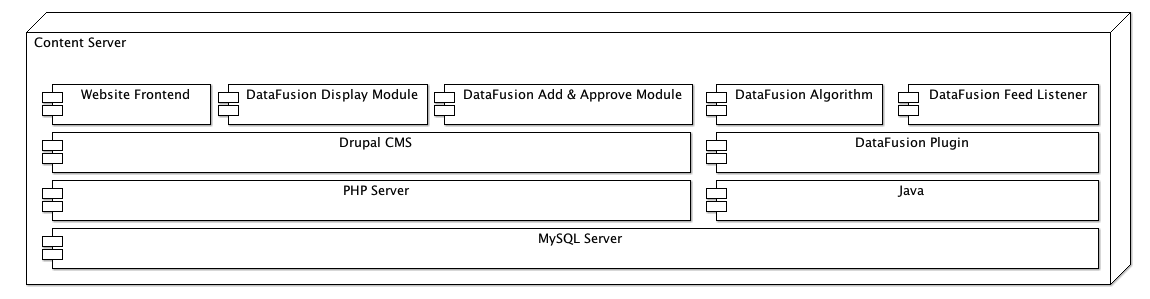
\includegraphics[width=6in]{images/software_stack}
\end{center}
\caption{The Software Stack}
\end{figure}

Amazon AWS’ CloudWatch will be used to handle automatic server scaling, elastic load balancing, and hosting of the servers. Soft state servers will be automatically launched by CloudWatch. These soft servers accept HTTP requests, check their internal memory based cache, if necessary makes HTTP requests to an external server to fill the cache, and returns the results of the HTTP requests. These servers will be stateless and be used to increase response time. The external server they request from will run the Drupal CMS and other applications.

\begin{figure}[h]
\begin{center}
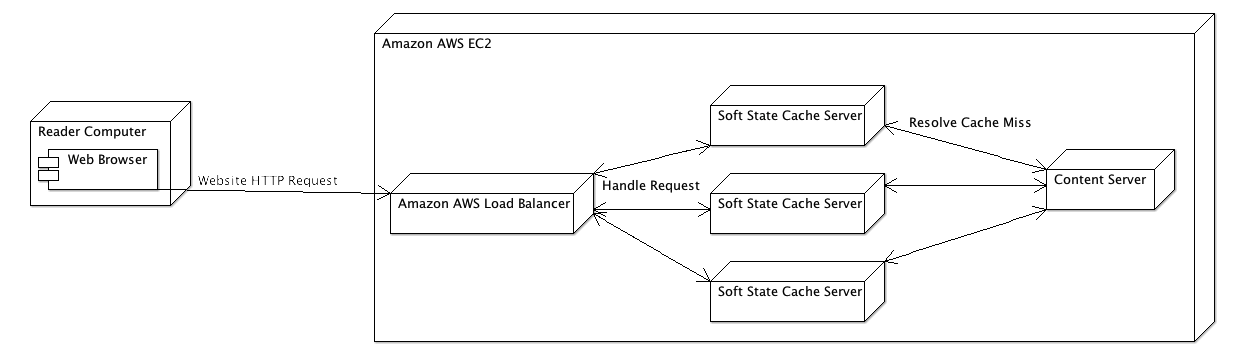
\includegraphics[width=6in]{images/data_flow}
\end{center}
\caption{The Data Flow}
\end{figure}

\subsection{Frameworks and Libraries}

At this stage of the project, the known frameworks and libraries are Drupal 7 CMS, Apache web server, and MySQL. Additional frameworks and libraries will be added to the project to take care of text parsing, machine learning, and other tasks.

\section{Planning}

The team has decided to follow an iterative design process in order to present our clients with prototypes at multiple stages during development.  Because the client has provided only a nebulous description of the project, we must elicit feedback early on to avoid diverging too far from the client’s expectations.  Our group will also benefits from being forced to create a functional, if simple, website early on; integration issues between the diverse parts of the project will be exposed before they become unmanageable.  Furthermore, getting the website to a working state every few weeks will provide a tangible and verifiable goal.

Our project involves both a traditional news website and more experimental data fusion, so we will borrow elements from the incremental software process as well.  In order to better develop largely independent elements such as a web scraper or learning algorithm, one or two group members will embark on a short “sprint” that is separate from the current iteration.  Once the “sprint” is complete, that work will be integrated back into the main system.

The only external stakeholders that the team will directly interact with is the client. As we have analyzed the availability and commitment of our client and found them to be good, we we will have no issues with external stakeholders.

The current management plan is to have two meetings a week. One meeting will be reserved to discuss logistics, team direction, and deal with overhead of the project. This will also include meeting with the client when necessary. The other meeting will be reserved for development. This will help speed development, ensure accountability and visibility, and ease integration.

The timetable, milestones, deliverables, and dates are shown below:
\begin{itemize}
 \item 09/21- Feasibility Study and Plan, Git Repository Created
 \item 10/11- Milestone 2
 	 \setlength{\itemindent}{5em}
	 \item Drupal Core Deployed to Development Server
	 \item Brand for Cornell Sun Tech Campus
	 \item User Interface (HTML, CSS)
	\setlength{\itemindent}{0em}
 \item 11/09- Milestone 3
	\setlength{\itemindent}{5em}
         \item Data Fusion Added
	 \item Web and RSS Feed storage
	 \item Automatic Data Fusion Algorithm
	\setlength{\itemindent}{0em}
 \item 12/07- Milestone 4
	\setlength{\itemindent}{5em}
	 \item Deployment to Amazon AWS
	 \item Performance and Mobile Optimization 
	 \item Demonstration and Handover
	\setlength{\itemindent}{0em}
\end{itemize}


\end{document}
